\documentclass[aspectratio=1610]{beamer}
\usepackage[utf8]{inputenc}
\usepackage{booktabs}
\usepackage{tabulary}
\usepackage{amssymb}% http://ctan.org/pkg/amssymb
\usepackage{pifont}% http://ctan.org/pkg/pifont
\newcommand{\cmark}{\ding{51}}%
\newcommand{\xmark}{\ding{55}}%
\usetheme{simple}
\usecolortheme{whiteonblack}
\title{Semantic MediaWiki}
\subtitle{Good for authoring Linked Data?}
\author{Konrad Höffner}

\begin{document}
\begin{frame}
\titlepage
\end{frame}

\begin{frame}{Situation: We generate large amounts of Linked Data}
\centering
\includegraphics[width=0.8\textwidth]{img/spider.png}
\end{frame}

\begin{frame}{Our data constantly changes}
\centering
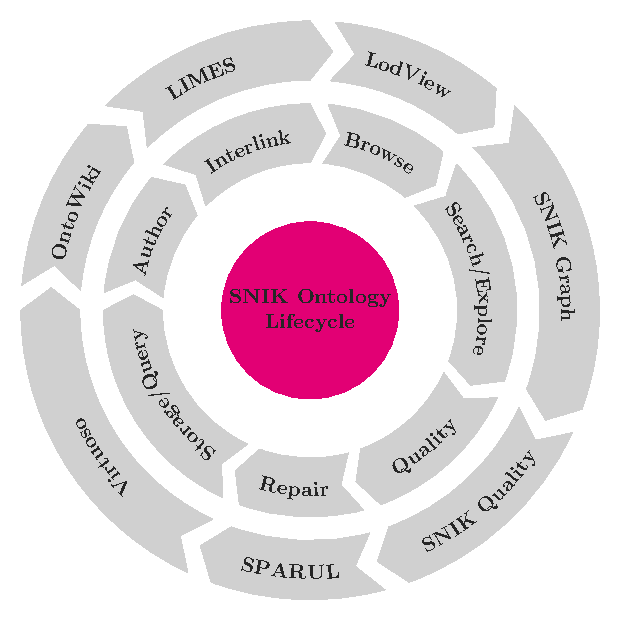
\includegraphics[height=0.9\textheight]{cycle.pdf}
\end{frame}

\begin{frame}{Problem: How to add, delete and modify Linked Data?}
\centering
\includegraphics[height=0.9\textheight]{cycle-red.pdf}
\end{frame}

\begin{frame}{Native Tools}
\centering
\begin{tabulary}{\textwidth}{lLL}
\toprule
Tool		&Advantages\\					
\midrule
Text Editor	&quick, small diffs, version control\\
SPARUL		&many changes at once, immediately available\\
\bottomrule
\end{tabulary}
\end{frame}

\begin{frame}{Problem solved?}
\centering
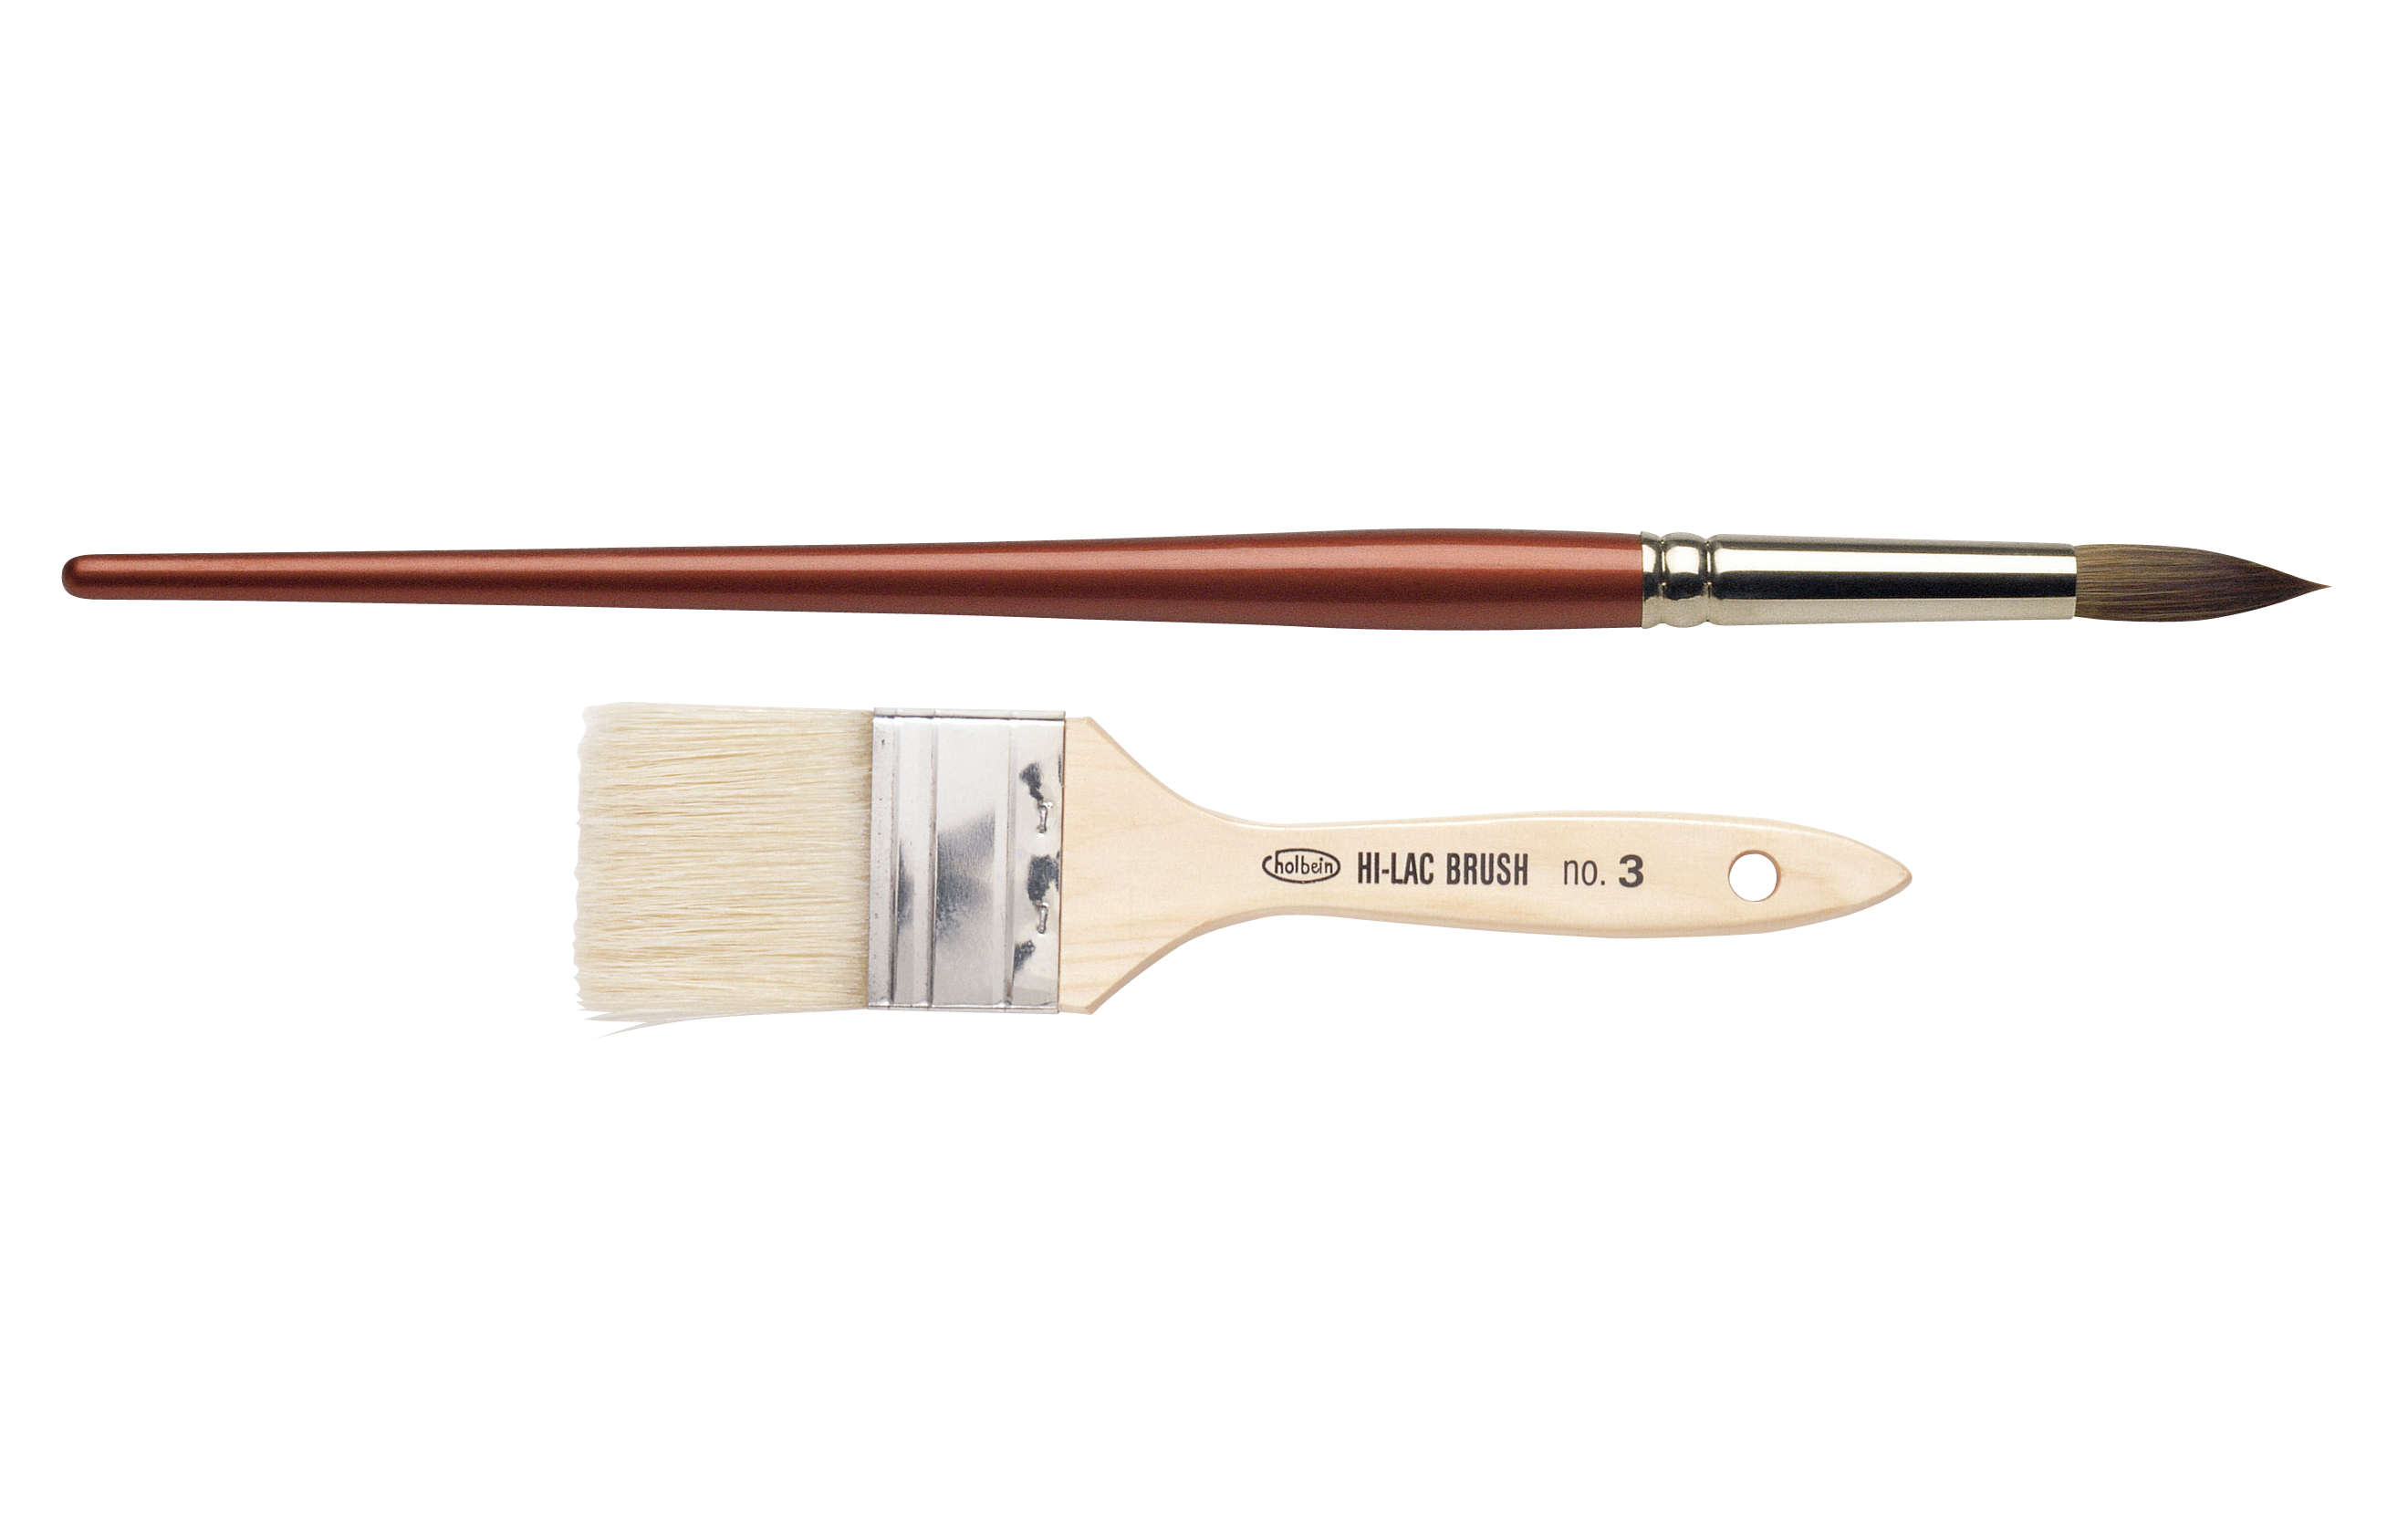
\includegraphics[width=0.9\paperwidth]{img/texteditorsparul.png}
\end{frame}

\begin{frame}{Unfortunately not}
\centering
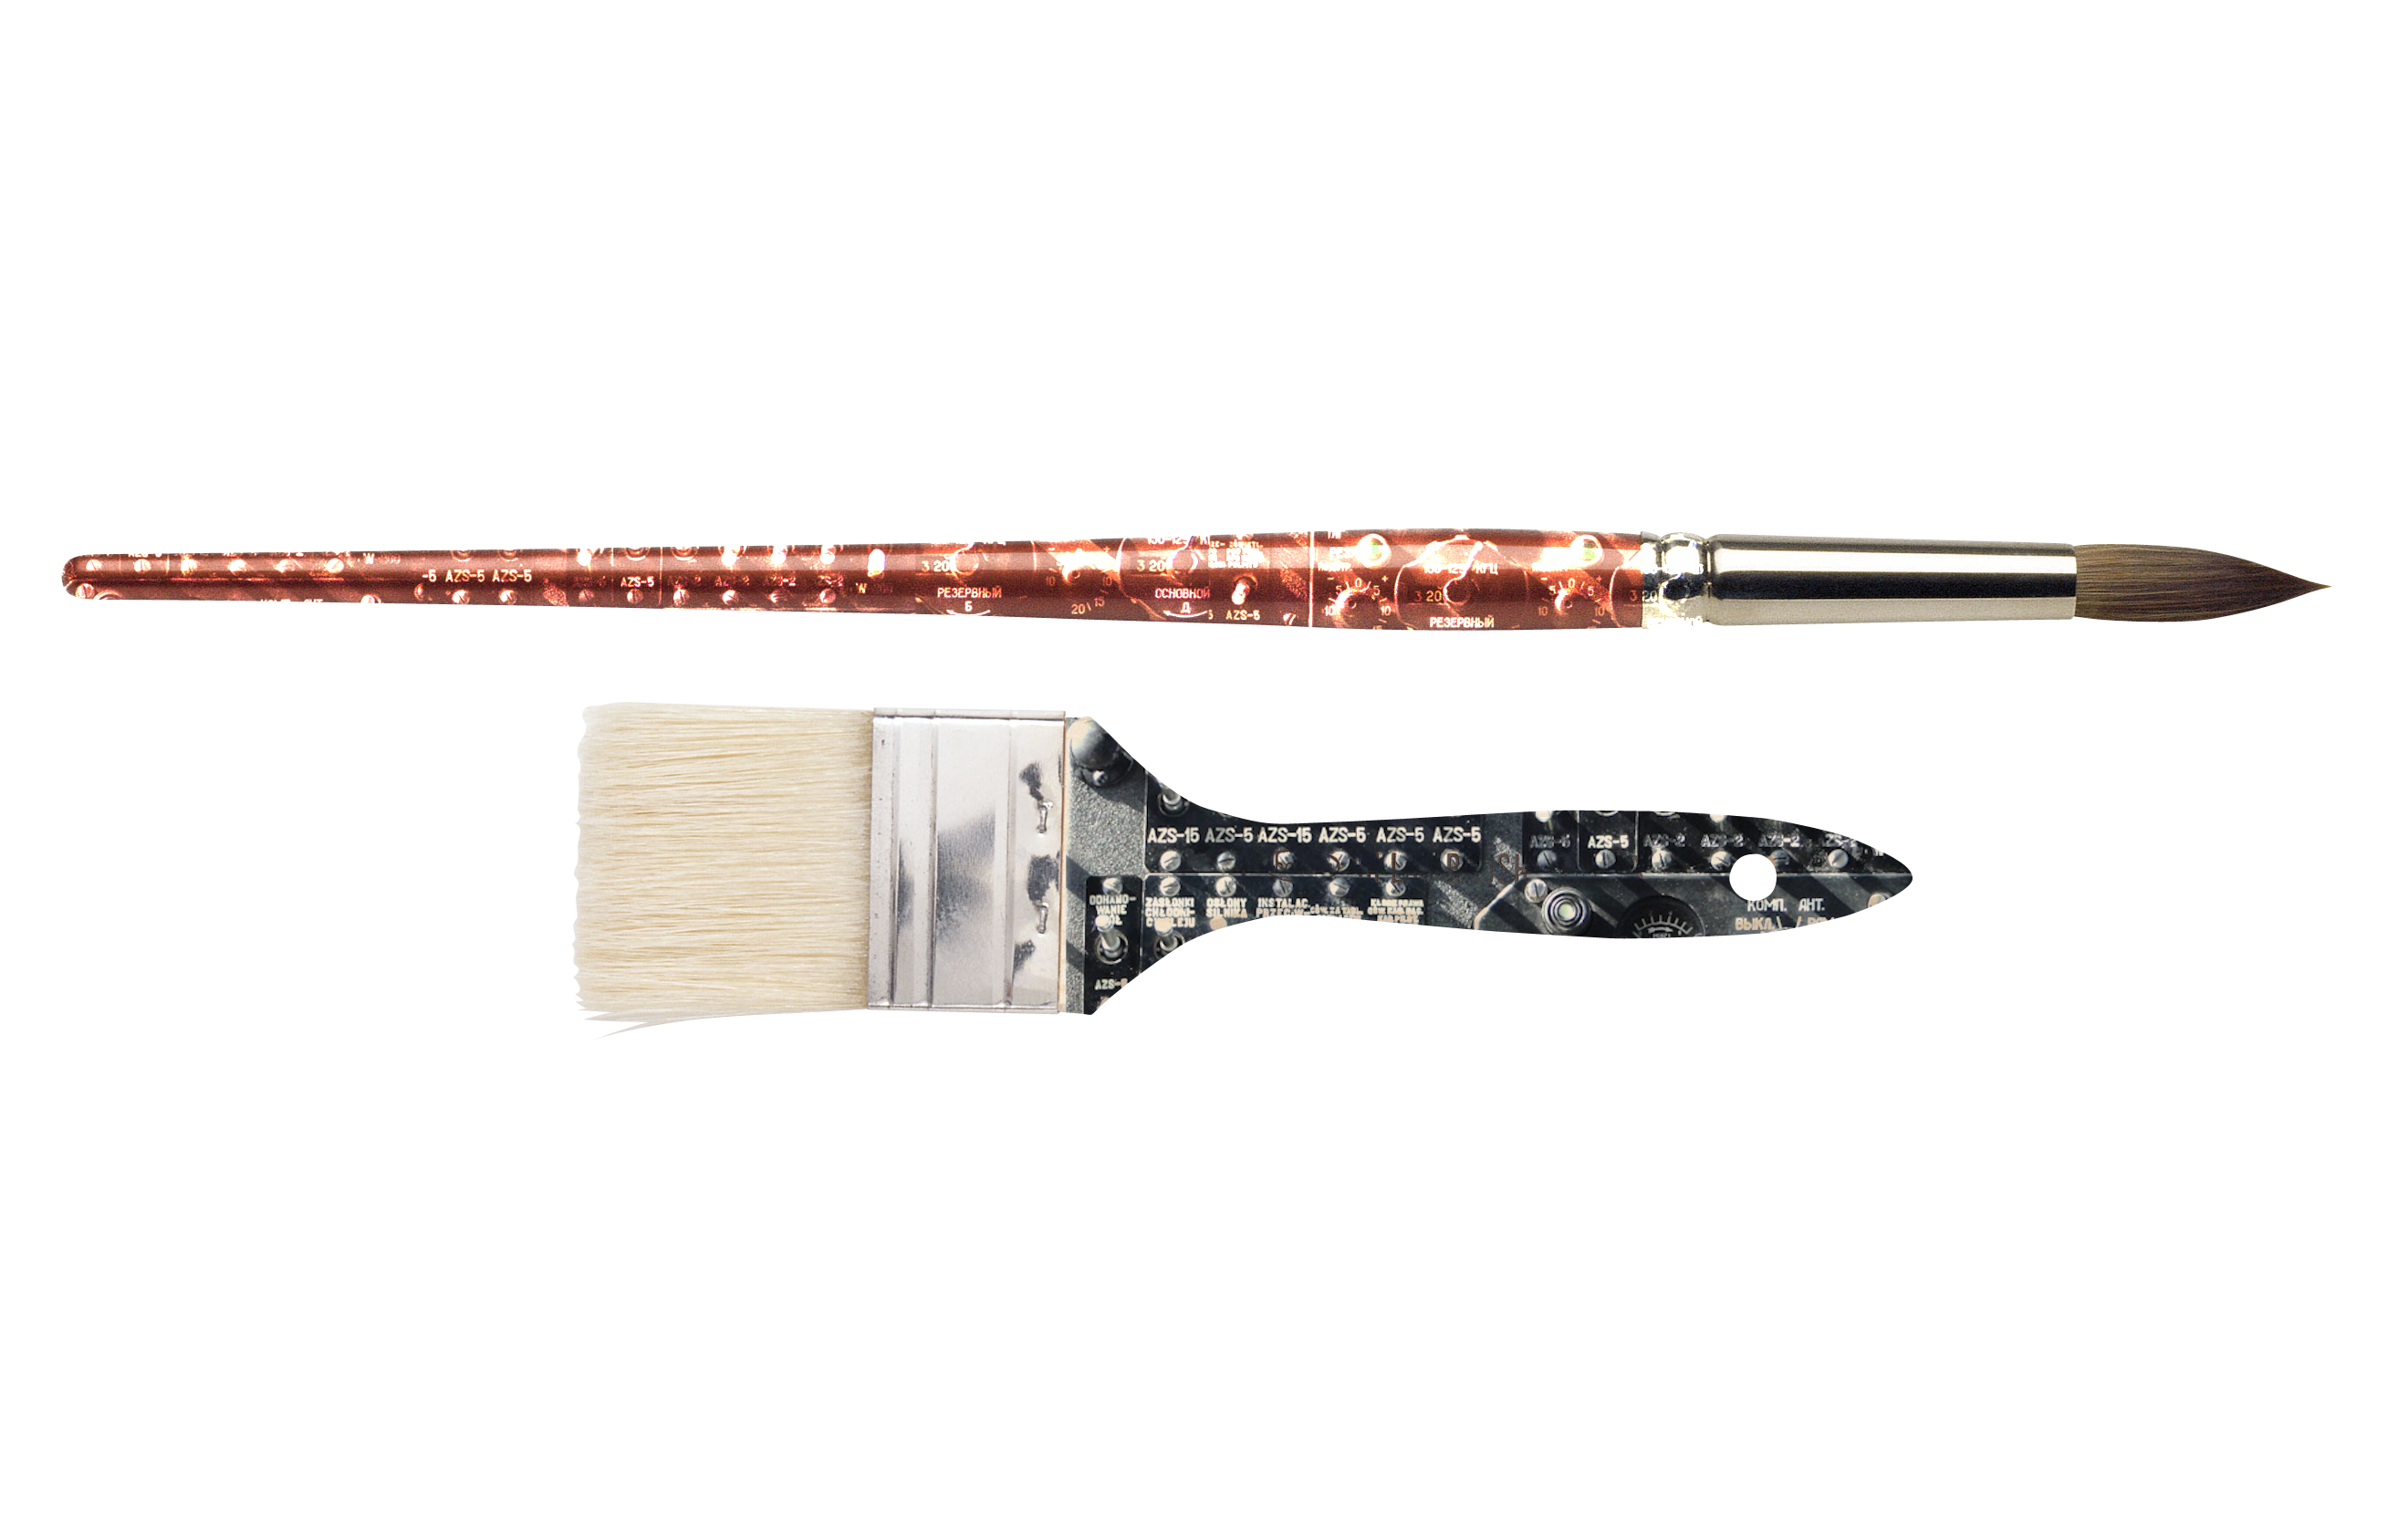
\includegraphics[width=0.9\paperwidth]{img/complicated.png}
\end{frame}

\iffalse
\begin{frame}{Problem: Authoring isn't easy}
\centering
\begin{tabulary}{\textwidth}{lLL}
\toprule
Tool		&Advantages						&Cons\\
\midrule
Text Editor	&speed, version control, 			&requires Turtle \& Git skills\\
SPARUL		&many changes at once 				&requires SPARUL syntax\\
Prot\'eg\`e	&\\
\bottomrule
\end{tabulary}
\end{frame}
\fi

\begin{frame}{User Interface: Prot\'eg\'e}
\centering
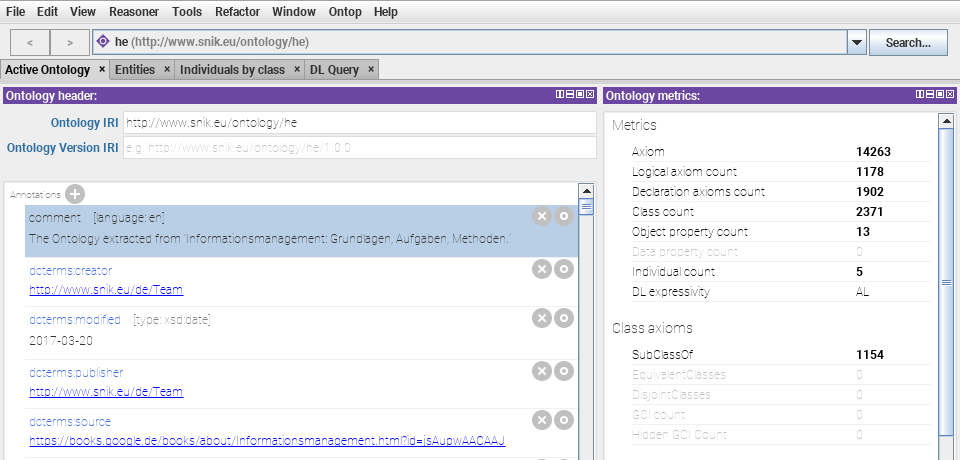
\includegraphics[width=0.6\paperwidth]{img/protege.png}
\begin{itemize}
\item large community
\item cannot use Virtuoso backend, even with WebProt\'eg\'e
\item optimized for OWL, not RDF
\end{itemize}
\end{frame}

\begin{frame}{User Interface: OntoWiki}
\centering
\includegraphics[height=0.7\textheight]{img/ontowiki.png}
\begin{itemize}
\item optimized for RDF, history, accounts
\item can use Virtuoso backend
\item productively used at IMISE
\item slow, cumbersome, not maintained anymore
\end{itemize}
\end{frame}

\begin{frame}{User Interface: Semantic MediaWiki}
\centering
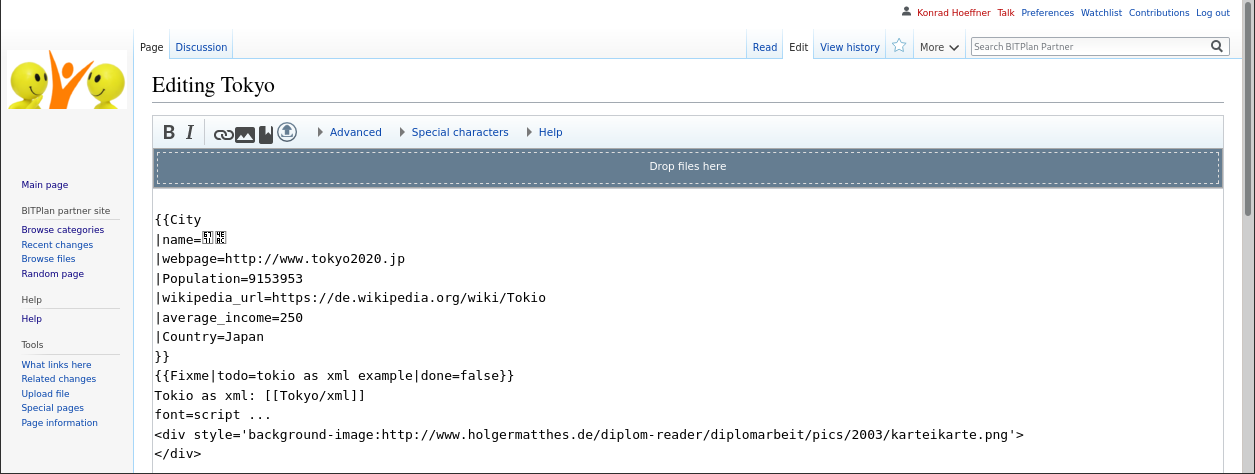
\includegraphics[width=0.6\paperwidth]{img/smw-tokyo.png}
\begin{enumerate}
\item what is the core idea?
\item can we use it to edit RDF?
\item is it user friendly? does it have enough functionality?
\item can it be integrated into our service infrastructure?
\item what is the environment, community and outlook?
\end{enumerate}
\end{frame}

\begin{frame}{Semantic MediaWiki---Core Idea}
\begin{itemize}
\item extension to MediaWiki (Wikipedia)
\item "store and query data within the wiki's page" 
\item hybrid between document and data
\item great fit for documents with data, but does it make sense for just data?
\end{itemize}
\end{frame}

\begin{frame}{Semantic MediaWiki---Edit RDF}
\begin{itemize}
\item typed links between documents
\item can be translated to RDF
\item PageForms extension to generate web forms with templates for a category $\rightarrow$ user generation of instances
\end{itemize}
\end{frame}

\begin{frame}[fragile]{Semantic MediaWiki---Usability}
\begin{verbatim}
{{#ask:
[[Kategorie:Stadt]]
[[Land::Schweiz]]
|?Name
|?Einwohner
}}
\end{verbatim}
\begin{itemize}
\item you need to check out for yourself whether it is usable for you
\item users need to learn Semantic MediaWiki syntax
\item we have a test account at an existing installation thanks to BITPlan
\item ask Konrad for credentials
\item be mindful, it is not our own instance
\end{itemize}
\end{frame}

\begin{frame}{Semantic MediaWiki---Integration}
\begin{itemize}
\item we use docker but all tested containers were broken
\item we use a Virtuoso SPARQL endpoint but there is no out-of-the box option to use Virtuso as a backend
\end{itemize}
\end{frame}

\begin{frame}{Semantic MediaWiki---Community and Outlook}
\begin{itemize}
\item thanks to Wolfgang Fahl of BITPlan for an introduction
\item 200-300 MediaWiki developers, focus on MediaWiki, rest of the world has to follow them
\item Semantic MediaWiki lacks unified leadership, many different fractions
\item usual data store are SQL databases and to a lesser extend wikiBase
\item very few users of SPARQL endpoints, no public example 
\end{itemize}
\end{frame}

\begin{frame}{Semantic MediaWiki---Summary}
\centering
\begin{tabulary}{\textwidth}{lL}
\toprule
Property		&Assessment\\
\midrule
Edit RDF		&~\\
Usability		&your assessment\\
Integration		&\xmark\\
Outlook			&\xmark\\
\midrule
Fit for our purposes	&\xmark\\
\bottomrule
\end{tabulary}
\end{frame}

\end{document}

